\section{Fragen}
\subsection*{1) Wieso ist die Annäherung für $\beta$ größer als $\pm40$ Grad nicht so gut?}
Zwischen $\beta=+40$ Grad und $\beta=-40$ Grad gibt es keine starken horizontalen Abweichungen bei der Bewegung des schwarzen Stabs. Die Bewegung ist hauptsächlich vertikal. Diese Bewegung kann linear gut approximiert werden. Nimmt $\beta$ Werte größer $40$ Grad, beziehungsweise kleiner $-40$ Grad an, wird die horizontale Auslenkung des schwarzen Stabs größer und die Approximation $\alpha=\frac{a_1}{a_2}\beta$ weicht immer stärker von der tatsächlichen Kurve $\alpha = f(\beta)$ ab. Der Graph verdeutlicht dies anschaulich.\\
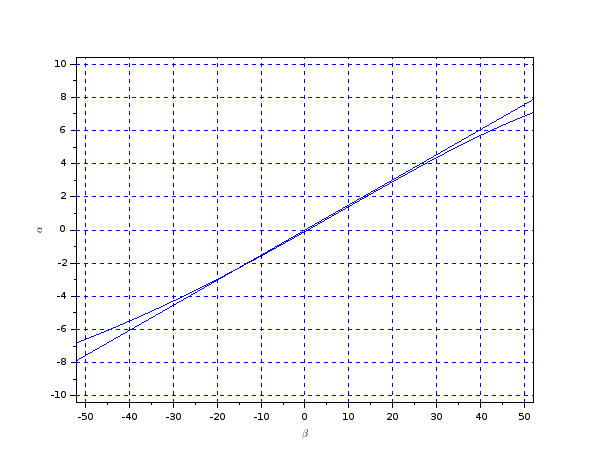
\includegraphics[scale=0.5]{images/plot1.png}

\subsection{2) $\beta = \pm 300$ Grad}
-periodisch